% !TeX root = prob.tex

\section{Ehrenfest Model and Two-State Process}\label{s.ehrenfest}

\textbf{Problem} The Ehrenfest model is designed to model diffusion of particles between two containers. In the following diagram there are four particles in the left container and six particles in the right container for a total of $n=10$ particles:
\begin{center}
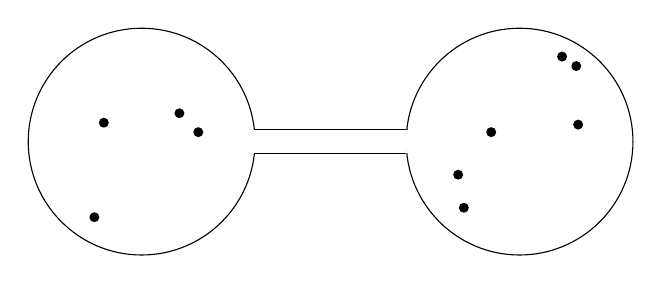
\begin{tikzpicture}[scale=1.2]
\draw (0,0) node {} circle[radius=1.2];
\draw[white,thick] (-6:1.2) arc(-6:6:1.2);
\draw (-6:1.2) -- +(1.63,0);
\draw (6:1.2) -- +(1.63,0);
\fill (-.4,.2) circle[radius=1.5pt];
\fill (.4,.3) circle[radius=1.5pt];
\fill (-.5,-.8) circle[radius=1.5pt];
\fill (.6,.1) circle[radius=1.5pt];
\begin{scope}[xshift=4cm]
\draw (0,0) node {} circle[radius=1.2];
\draw[white,thick] (174:1.2) arc(174:186:1.2);
\fill (-.3,.1) circle[radius=1.5pt];
\fill (.45,.9) circle[radius=1.5pt];
\fill (-.65,-.35) circle[radius=1.5pt];
\fill (.62,.18) circle[radius=1.5pt];
\fill (-.59,-.7) circle[radius=1.5pt];
\fill (.6,.8) circle[radius=1.5pt];
\end{scope}
\end{tikzpicture}
\end{center}
Repeated choose a particle at random with uniform distribution and move it to the other container. If there are $i$ particles in the left container then the probability of choosing a particle from the left container is $i/n$ and the probability of choosing a particle from the right container is $(n-i)/n$. If one container is empty the next particle must be chosen from the other container. 

The problem is similar to the gambler's ruin except that: (a) the process never ends and (b) the probability of a left or right step changes with each step:
\begin{center}
\begin{tikzpicture}[scale=1.2]
\draw (0,0) node[above left] {$A$} -- 
      (10,0) node[above right] {$B$};
\foreach \x in {0,1,2,3,4,5,6,7,8,9,10} {
  \draw (\x,0) -- +(0,4pt);
  \node at (\x,-10pt) { $\x$ };
}
\node at (4,-9mm) {$i$};
\node at (10,-9mm) {$n$};
\draw[fill] (4,7mm) circle[radius=1pt];
\draw[->] (4,7mm) -- node[above] {$\disfrac{n-i}{n}$} +(-1,0);
\draw[->] (4,7mm) -- node[above] {$\disfrac{i}{n}$} +(1,0);
\draw[->] (0,7mm) -- node[above] {$1$} +(1,0);
\draw[<-] (9,7mm) -- node[above] {$1$} +(1,0);
\end{tikzpicture}
\end{center}

\subsection{Theoretical results}

The process is a \emph{Markov chain}. Eventually, the process will reach a \emph{stationary distribution}:
\[
s_i=\dischoose{n}{i}\left(\frac{1}{n}\right)^n\,,
\]
where $s_i$ is the proportion of time that the particle is at the $i$'th position.

\subsection{Program structure}

\verb+configuration.py+ contains declarations of variables which are intended to be constant. 

\verb+ehrenfest_plot.py+ contains the functions for plotting the distribution, both the theoretical distribution and the result of the simulation.

\verb+ehrenfest.py+ is the main program which obtains the parameter $n$, runs the simulations, prints the output and calls the plotting functions.

\subsection{Running the simulations}

The program asks the user how to run the simulation: with the saved value of $n$ or with a new value of $n$. Here is an output of the simulation:
\begin{verbatim}
Total particles in urns = 10
Theoretical stationary distribution
[0.001 0.01  0.044 0.117 0.205 0.246 0.205 0.117 0.044 0.01  0.001]
Simulation stationary distribution
[0.001 0.009 0.044 0.12  0.208 0.243 0.205 0.121 0.042 0.008 0.001]
\end{verbatim}
A graph of these distributions is shown in Figure~\ref{f.ehrenfest1}; the theoretical distribution and the result of simulation are so close together that the lines are slightly offset.

\begin{figure}
\begin{center}
\includegraphics[width=\textwidth]{ehrenfest-01}
\caption{Stationary distribution for the Ehrenfest model}\label{f.ehrenfest1}
\end{center}
\end{figure}

\newpage

\subsection{The two-state process}

The two-state process is similar to the Ehrenfest model in that the probabilities at each step are different and we are interested in the stationary probability distribution of the unbounded process.

There are two states $A,B$. When the process is in state $A$, with probability $a$ it transitions to $B$ and with probability $1-a$ it remains in $A$. Similarly, the probability of a transition from $B$ to $A$ is $b$:
\begin{center}
\begin{tikzpicture}[->,node distance = 6mm and 2cm]
\node[draw,circle,minimum size=10mm] (A) {$A$};
\node[draw,circle,minimum size=10mm] (B) [right=of A] {$B$};
\draw (A) edge[bend left] node[above] {$a$} (B);
\draw (B) edge[bend left] node[below] {$b$} (A);
\draw (A) edge [loop left] node {$1-a$} (A);
\draw (B) edge [loop right] node {$1-b$} (B);
\end{tikzpicture}
\end{center}

The stationary distribution is:
\[
\left[\frac{b}{a+b}, \frac{a}{a+b}\right]\,.
\]

Here is an output of the simulation:
\begin{verbatim}
Probabilities:  a = 0.500, b = 0.333
Theoretical stationary distribution: a = 0.400, b = 0.600
Simulation  stationary distribution: a = 0.402, b = 0.598
\end{verbatim}
